%%% LaTeX Template
%%% This template can be used for both articles and reports.
%%%
%%% Copyright: http://www.howtotex.com/
%%% Date: February 2011

%%% Preamble
\documentclass[paper=a4, fontsize=11pt]{scrartcl}	% Article class of KOMA-script with 11pt font and a4 format
\usepackage[margin=0.7in]{geometry}
\usepackage[english]{babel}															% English language/hyphenation
\usepackage[protrusion=true,expansion=true]{microtype}				% Better typography
\usepackage{amsmath,amsfonts,amsthm}										% Math packages
\usepackage[pdftex]{graphicx}														% Enable pdflatex
%\usepackage{color,transparent}													% If you use color and/or transparency
\usepackage[hang, small,labelfont=bf,up,textfont=it,up]{caption}	% Custom captions under/above floats
\usepackage{epstopdf}																	% Converts .eps to .pdf
\usepackage{subfig}																		% Subfigures
\usepackage{booktabs}																	% Nicer tables

%%% Advanced verbatim environment
\usepackage{verbatim}
\usepackage{fancyvrb}
\DefineShortVerb{\|}								% delimiter to display inline verbatim text


%%% Custom sectioning (sectsty package)
\usepackage{sectsty}								% Custom sectioning (see below)
\allsectionsfont{%									% Change font of al section commands
	\usefont{OT1}{bch}{b}{n}%					% bch-b-n: CharterBT-Bold font
%	\hspace{15pt}%									% Uncomment for indentation
	}

\sectionfont{%										% Change font of \section command
	\usefont{OT1}{bch}{b}{n}%					% bch-b-n: CharterBT-Bold font
	\sectionrule{0pt}{0pt}{-5pt}{0.8pt}%	% Horizontal rule below section
	}


%%% Custom headers/footers (fancyhdr package)
\usepackage{fancyhdr}
\pagestyle{fancyplain}
\fancyhead{}														% No page header
\fancyfoot[C]{\thepage}										% Pagenumbering at center of footer
\renewcommand{\headrulewidth}{0pt}				% Remove header underlines
\renewcommand{\footrulewidth}{0pt}				% Remove footer underlines
\setlength{\headheight}{13.6pt}

%%% Equation and float numbering
\numberwithin{equation}{section}															% Equationnumbering: section.eq#
\numberwithin{figure}{section}																% Figurenumbering: section.fig#
\numberwithin{table}{section}

\usepackage[parfill]{parskip}
\usepackage{float}
\usepackage{graphicx}
\usepackage{hyperref}
\usepackage[numbers]{natbib}															% Tablenumbering: section.tab#



%%% Title	
\title{ \vspace{-1in} 	\usefont{OT1}{bch}{b}{n}
		\huge \strut Vesuvio Data Reduction and Analysis in Mantid \strut \\
}
\author{ 									\usefont{OT1}{bch}{m}{n}
        Samuel Jackson\\		\usefont{OT1}{bch}{m}{n}
        ISIS Facility\\	\usefont{OT1}{bch}{m}{n}
        Rutherford Appleton Laboratory\\
        \texttt{samuel.jackson@stfc.ac.uk}
}
\date{\today}

%%% Begin document
\begin{document}
\maketitle
\clearpage
\tableofcontents
\clearpage
\section{Introduction}
\label{sec:introduction}
VESUVIO is an neutron spectrometer at the ISIS pulsed neutron source operating a high energy range of between 5-150 eV and uses the experimental technique known as neutron Compton scattering to measure the momentum distributions of condensed matter systems \citep{mayers2012vesuvio}. It is located on the S2 beamline and features 64 forward scattering Yttrium Aluminium Perovskite (YAP) $\gamma$-ray detectors and 132 $^{6}$Li doped glass scintillator neutron detectors \citep{mayers2011calibration}.

Mantid \citep{mantid} is a data analysis application for neutron and muon scattering data used by multiple facilities across the world. Recently, extensive work has been carried out to integrate the bespoke data reduction and analysis routines with the Mantid framework. While the programs described in this document are designed to replicate the functionality of the Fortran and Genie routines already in use, most of them have been written from scratch and are not based on the original code base. This document outlines the current progress of development regarding what has already been implemented and what is remains to be finished.

\section{Vesuvio Overview}
Vesuvio is a deep inelastic neutron scattering spectrometer situated on the S2 beamline at ISIS with an operational energy range of 5-150 eV. The instrument utilises a indirect geometry design with the final energy being fixed at 4.89 eV \cite{mayers2011calibration} and consists of 64 Yttrium Aluminium Perovskite $\gamma$-ray forward scattering detectors in 8 separate banks and 132 $^6$Li doped glass scintillator back scattering detectors split into 3 banks. The final energy for both forward and back scattering detectors are determined using gold foils which have a large resonance peak at 4.9 eV $\pm$ 0.15 eV. 

\begin{figure}[H]
\centering
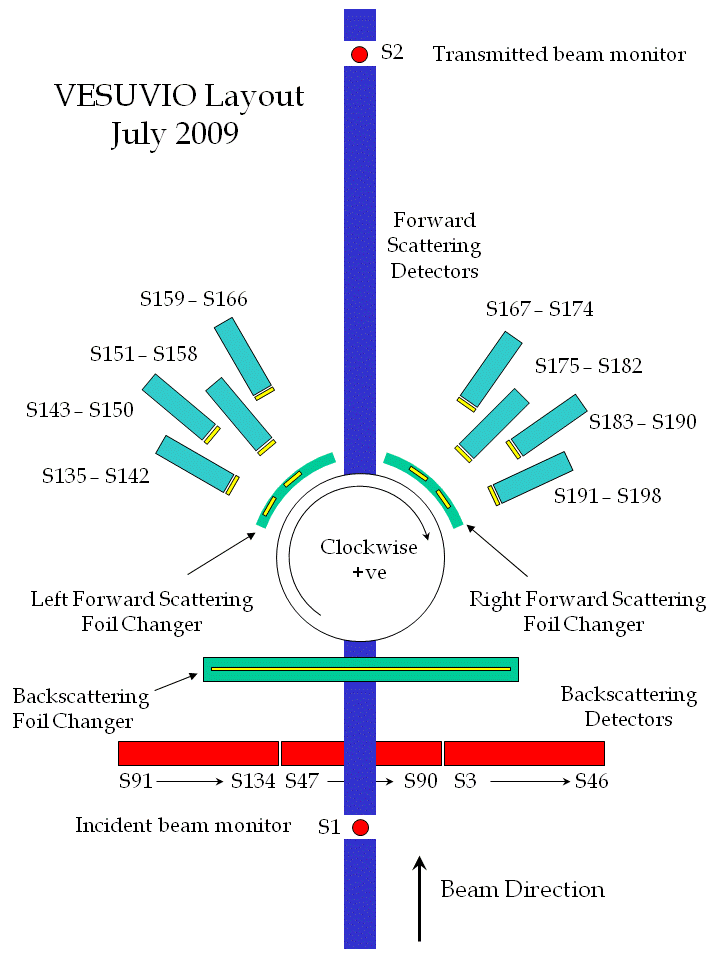
\includegraphics[width=0.5\textwidth]{img/vesuvio-diagram.png}
\caption{Schematic diagram of the Vesuvio instrument. Positions of the gold foils used for each of the differencing methods are shown in yellow.}
\label{fig:vesuvio-diagram}
\end{figure}

The forward scattering detectors make use of the difference technique described in Ref. \cite{schooneveld2006foil} which use the gold foils both as detectors and energy selectors by detecting the $\gamma$-ray cascade emitted when a neutron is absorbed. The back scattering detectors utilise a similar process but use a double differencing technique described in Ref. \cite{seeger1985double}.

Vesuvio is primarily designed to measure the atomic momentum distribution of atoms in condensed matter systems. Data analysis on Vesuvio relies on the accuracy of the impulse approximation which implies that for incident neutron wavelengths much less than the $d$-spacing of the sample, atoms will scatter incoherently and the measured intensity is therefore the total sum of intensities for individual atoms in the sample \cite{fernandezalonso2013neutron}. This effectively treats the scattering as a single atom 'billiard ball', with conservation of momentum and kinetic energy of a neutron a single target atom, allowing the momentum distribution of a mass to be measured using the theory developed in Ref. \cite{mayers2004vesuvio}.

The resulting time-of-flight data contains a number of spectra each consisting of a series of peaks. Each of these peaks corresponds to a single atomic mass in the sample begins studied. The positions of the peaks in the spectrum are determined by the mass of the sample. The amplitude of each of the peaks is determined by an atoms mass and scattering cross section. Finally, the width of the peaks is determined by the momentum distribution of the mass. The goal of data analysis of Vesuvio data is to determine the shape and intensity of the peaks, thereby determining the momentum distributions of the atoms in the sample. \cite{mayers2010user}.

\section{Introduction to the Vesuvio Data Analysis Package}
\label{sec:intro-data-analysis}
The Mantid development team in combination with Vesuvio instrument scientists have created a data analysis package to help aid with the analysis of Vesuvio data. This is still under heavy development and is currently in the form of a separate python module called ncs.py (NCS: Neutron Compton Scattering) which provides a collection of help functions for data analysis which builds upon the existing Mantid framework. This module is currently available in the Mantid Github scripts repository in the \textit{development \textgreater  inelastic} folder \cite{mantidgithubncs}.

\section{Viewing Data in Time-of-Flight}
\label{sec:viewtof}
The original data analysis package \cite{mayers2010user} used two separate commands to process the raw time-of-flight data, one for the front scattering detectors and one for the back scattering. In the Mantid implementation this has been replaced with a single algorithm called LoadVesuvio which performs all of the processing for raw files from the instrument. This includes options for handling each of the different foil positions and difference techniques available with Vesuvio \citep{schooneveld2006foil, mayers2004vesuvio} and handles the summing multiple runs. It also contains a flag for summing each spectrum in the desired range into a single spectrum. The results of this loading operation are output as a single workspace in Mantid with units in time-of-flight which can be plotted using Mantid's various visualisation tools.

\begin{figure}[H]
\centering
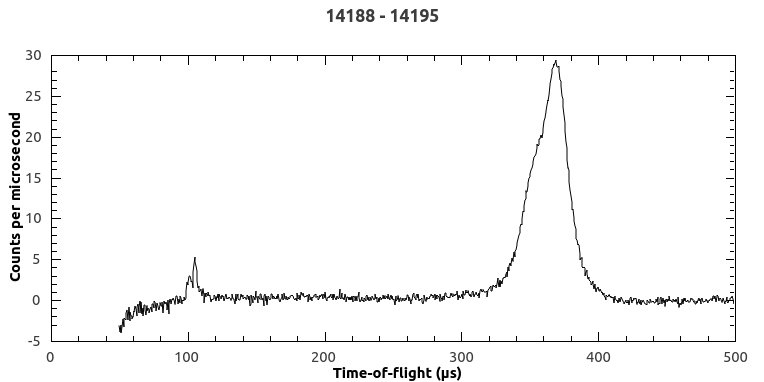
\includegraphics[width=0.6\textwidth]{img/tof-spectrum.png}
\caption{Plot of time-of-flight data from the sum runs 14188-14195 and the sum of detectors 40-134.}
\label{fig:tof-spectrum}
\end{figure}

Optionally, an instrument parameter file can be supplied to the loading routine. This file contains a set of calibrated instrument parameters for each of the detectors and can correct each of the default parameters used and attach $t0$ (the time delay offset parameter) \cite{mayers2011calibration} to the instrument attached to the workspace. This parameter file is usually generated by the instrument scientist using a set of reference runs using the calibration program outlined in section \ref{sec:calibration} and does not need to be regenerated for every analysis session. 

Once a Vesuvio data has been loaded into a Mantid workspace it can be used with the various tools in the ncs data analysis module. Typically the first step after loading the raw data in time-of-flight is to crop the workspace to a sensible range for data analysis. This can be done by using the Mantid CropWorkspace algorithm. The typically time-of-flight range used is 50.0 - 562.0 $\mu s$.

The ncs.py module also provides a preprocessing function for further preparing the data for analysis. This method provides options for masking data points in the raw workspace given an error threshold as well as an option to smooth the workspace using the SmoothData algorithm.

\section{Multiple Scattering and Gamma Background Corrections}
\label{sec:corrections}
The time-of-flight data loaded using the methods described in section \ref{sec:viewtof} need to be corrected to account for the effects of multiple scattering \citep{mayers2002multiple} and gamma background \citep{mayers2011calculation}. Currently, the multiple scattering corrections for VESUVIO in Mantid are uder development and will be available in future release cycles.

Corrections for the gamma background are implemented using the Mantid algorithm framework as an algorithm called CalculateGammaBackground. This takes a single workspace in time-of-flight, and a fit function describing the mass spectrum of the input data and a list of workspace indices to include as part of the correction. The fit function for the mass spectrum is typically one which has been created as part of the fit routines described in section \ref{sec:fitting}. This algorithm results in two workspaces: one that contains the calculated background and a copy of the input time-of-flight workspace with the background subtracted.

\begin{figure}[H]
\centering
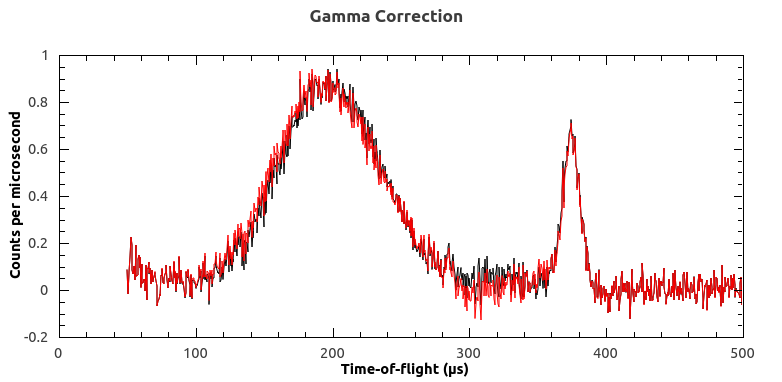
\includegraphics[width=0.6\textwidth]{img/corrections-gamma.png}
\caption{Plot of a Zirconium Hydride (ZrH$_2$) sample. Black is the uncorrected sample, red shows the same sample after gamma correction.}
\label{fig:corrections-gamma}
\end{figure}

Again, there are helper functions for this implemented in ncs.py. The gamma background can be computed from a workspace simply by using the \textit{gamma\_correct} function and passing the workspace to correct, the required fitting options, and the parameters produced from a fit (see section \ref{sec:fitting}).

\section{Fitting}
\label{sec:fitting}
The majority of the development for integrating Vesuvio into Mantid has concerned the development of the fitting procedures required to measure the neutron compton profile following the theory described in Ref.\citep{mayers2012vesuvio}. Development in this area has focussed on two major additions to the Mantid framework. First was the creation a new suite of fit functions was required which could accurately describe the results of a neutron Compton scattering experiment. The second was the creation of a collection of supporting data analysis functions which allow the user to easily setup a fit given the appropriate parameters for the sample and are available in the ncs.py module.

\begin{figure}[H]
\centering
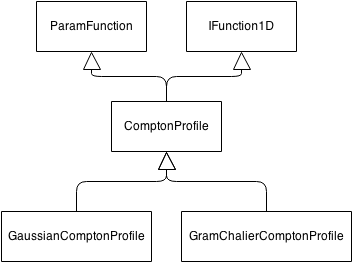
\includegraphics[width=0.4\textwidth]{img/uml/compton-class-diagram.png}
\caption{Class diagram of the Compton Profile fit functions in Mantid.}
\label{fig:compton-class-diagram}
\end{figure}

There are two major fit functions used in the analysis of Vesuvio data. The GaussianComptonProfile defines a function for fitting the simpler Gaussian approximation to mass peaks. The GramChalierComptonProfile is for the more complex fitting case where the atoms in the sample are affected by anisotropy and anharmonicity. Both of these are described in detail in Refs. \citep{mayers2012vesuvio}.

Both of these fit functions inherit from a common class called the ComptonProfile. This implements the common operations between both fit functions such as conversion of time-of-flight data to y-space and the calculation of the resolution components.


\section{Diffraction}
\label{sec:diffraction}
Diffraction on VESUVIO is not yet fully implemented within Mantid. As the reduction of diffraction data is fairly trivial in comparison to the other requirements of VESUVIO data analysis, this can be handled by the existing IndirectDiffractionReduction routine that is used as part of the 

\section{Calibration}
\label{sec:calibration}

\section{GUI}
\label{sec:GUI}

\section{Visualisation}
\label{sec:visualisation}


\bibliographystyle{unsrtnat_corrected}
\bibliography{references}
\end{document}